% Multiple Choice Question 24

\begin{questions}
\setcounter{question}{23}

\question
A long, straight wire of radius $R$ carries current $I$. The current is distributed over the cross-sectional area of the wire with a uniform current density. Which of the following graphs best represents the magnetic field strength produced by the current as a function of the distance $r$ from the center of the wire?

\begin{oneparchoices}
    \choice \adjustbox{valign=t}{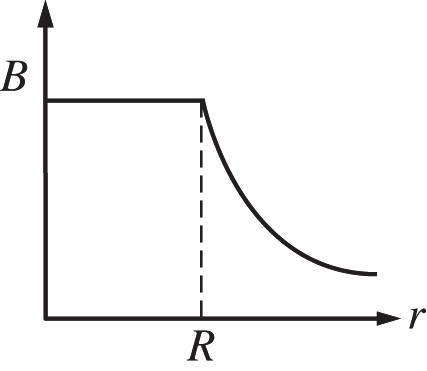
\includegraphics[scale=0.3]{images/img-011-014.png}}
    \choice \adjustbox{valign=t}{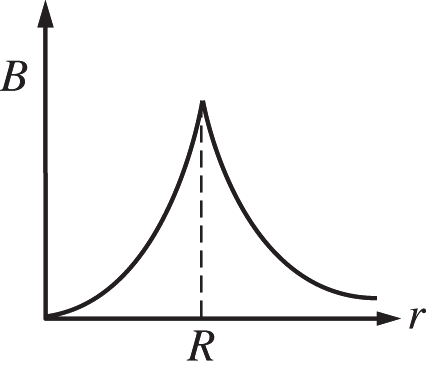
\includegraphics[scale=0.3]{images/img-011-015.png}}
    \choice \adjustbox{valign=t}{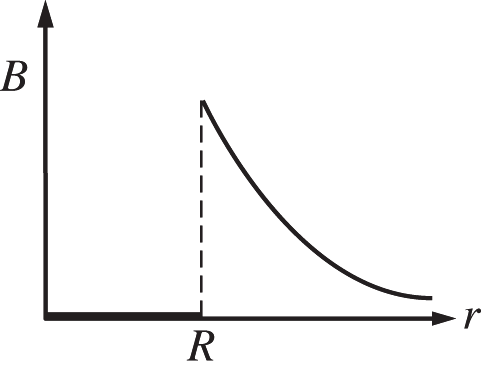
\includegraphics[scale=0.3]{images/img-011-016.png}}
    \choice \adjustbox{valign=t}{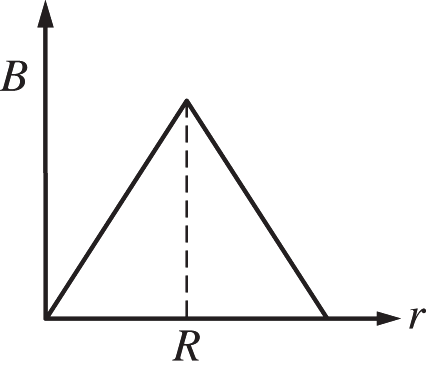
\includegraphics[scale=0.3]{images/img-011-017.png}}
    \choice \adjustbox{valign=t}{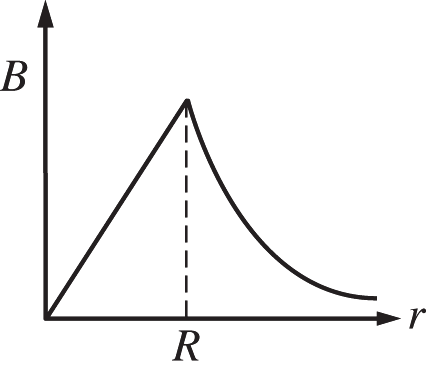
\includegraphics[scale=0.3]{images/img-011-018.png}}
\end{oneparchoices}

\end{questions}
